\section{Serangan Pasif vs Serangan Aktif}
\label{sec:pasif-aktif}

Berdasarkan keterlibatan penyerang dalam komunikasi, serangan dibagi menjadi dua
kelas besar. Pembagian ini penting karena berimplikasi langsung pada cara
penanganannya: serangan pasif tidak dapat dideteksi, sehingga pencegahannya harus
bersifat preventif, sedangkan serangan aktif dapat dideteksi, sehingga
penanganannya dapat bersifat reaktif.

\subsection{Serangan Pasif (\textit{Passive Attack})}

Penyerang tidak mengubah data atau terlibat aktif dalam komunikasi; ia hanya
menyadap informasi. Enkripsi pesan mencegah penyadap memahami isi pesan, tetapi
enkripsi tidak menghilangkan seluruh jejak: keberadaan, waktu, dan volume
komunikasi tetap terlihat. Dua bentuk serangan pasif yang lazim adalah:
\begin{itemize}
    \item \textbf{Intersepsi} (\textit{interception}): menyadap konten pesan.
          Gambar~\ref{fig:serangan-pasif-intersepsi} menampilkan situasinya.
    \item \textbf{Analisis lalu lintas} (\textit{traffic analysis}): mengamati pola
          lalu lintas data --- siapa berkomunikasi dengan siapa, kapan, dan berapa
          banyak data yang dikirim --- tanpa perlu membaca isinya, seperti pada
          Gambar~\ref{fig:serangan-analisis-lalu-lintas}.
\end{itemize}

Analisis lalu lintas sering diremehkan, padahal dalam banyak situasi polanya saja
sudah sangat informatif. Bahwa sebuah kantor notaris menghubungi seorang ahli waris
tengah malam, atau bahwa sebuah perusahaan mengirimkan data berukuran sangat besar
tepat sebelum pengumuman kuartalan, adalah informasi berharga meskipun isi
pesannya tersandi rapat. Karena itulah, sistem yang serius tidak hanya
mengenkripsi isi pesan tetapi juga menyamarkan pola lalu lintasnya, misalnya dengan
selalu mengirim paket berukuran tetap pada selang waktu tetap.

\begin{figure}[htbp]
    \centering
    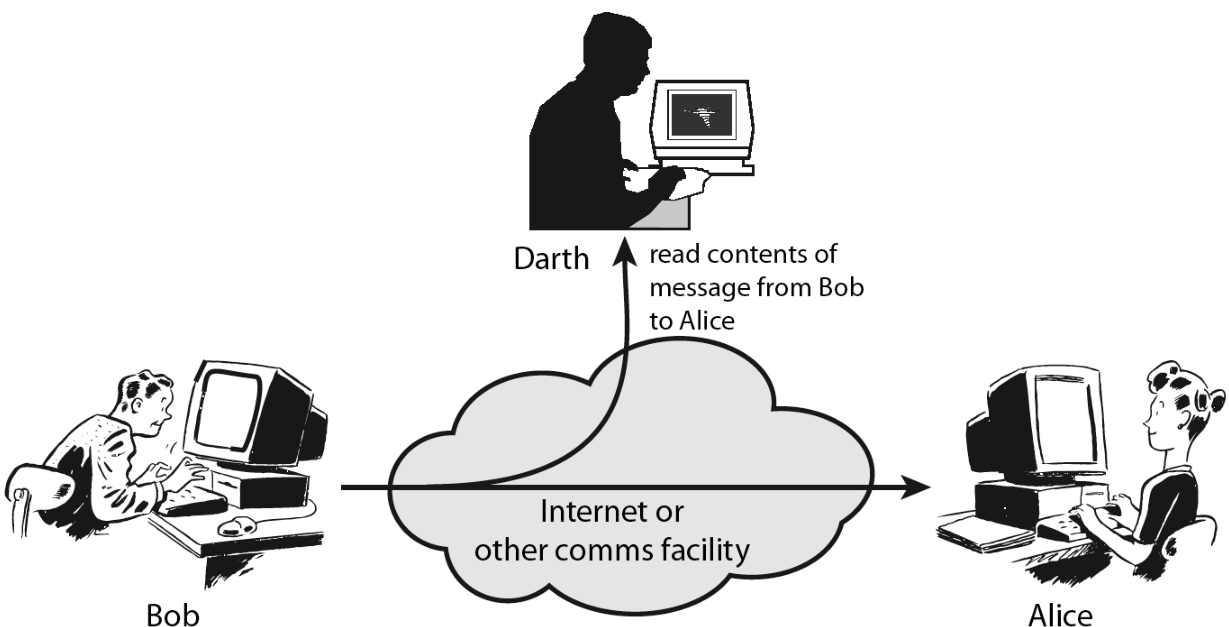
\includegraphics[width=0.78\linewidth, height=0.7\textheight, keepaspectratio]{figures/serangan-pasif-intersepsi.png}
    \caption{Serangan pasif berupa intersepsi: penyerang menyadap dan membaca isi pesan yang melintas di jaringan tanpa mengubahnya}
    \label{fig:serangan-pasif-intersepsi}
    \sumber{Munir, \textit{IF4020 Kriptografi}, ITB.}
\end{figure}

\begin{figure}[htbp]
    \centering
    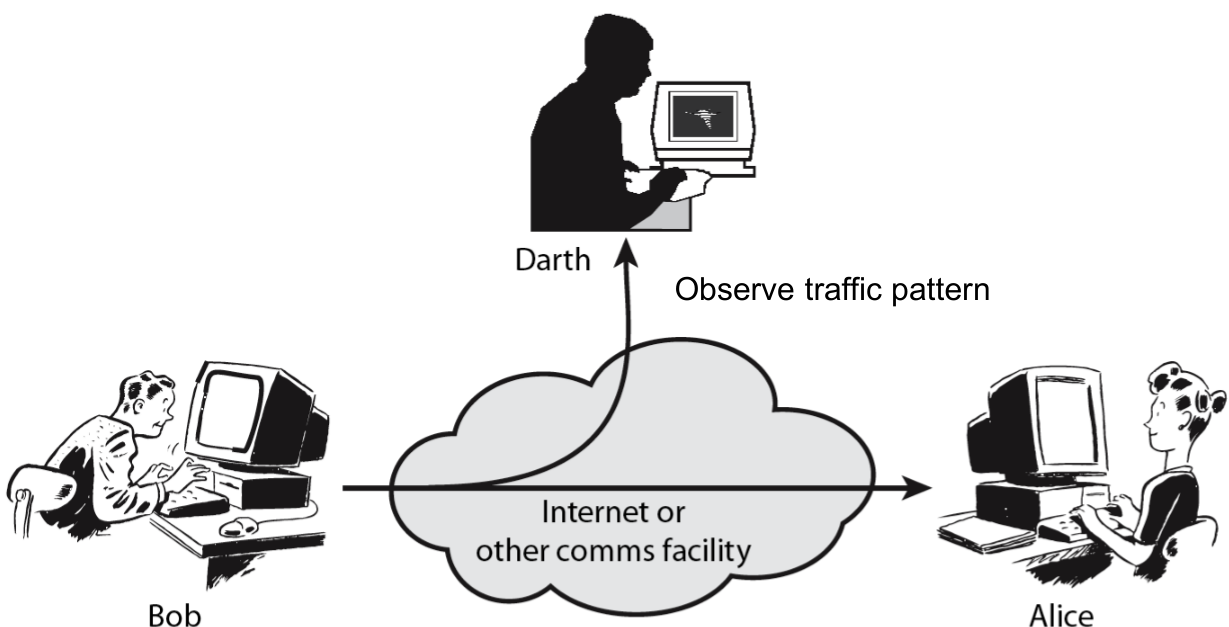
\includegraphics[width=0.78\linewidth, height=0.6\textheight, keepaspectratio]{figures/serangan-analisis-lalu-lintas.png}
    \caption{Serangan pasif berupa analisis lalu lintas: penyerang tidak membaca isi pesan, melainkan mengamati pola siapa berkomunikasi dengan siapa, kapan, dan seberapa besar datanya}
    \label{fig:serangan-analisis-lalu-lintas}
    \sumber{Munir, \textit{IF4020 Kriptografi}, ITB; diadaptasi dari Stallings.}
\end{figure}

\subsubsection{Alat dan Metode Penyadapan}

Perkakas analisis lalu lintas seperti \textbf{Wireshark} dapat digunakan untuk
memantau lalu lintas jaringan. Bila data tidak dienkripsi, penyadap tidak perlu
menganalisis apa pun: nama pengguna dan kata sandi langsung terbaca pada tangkapan
paket, seperti diperlihatkan Gambar~\ref{fig:wireshark-plaintext}. Contoh ini
sekaligus menjelaskan mengapa protokol yang mengirim kata sandi dalam bentuk
terbuka --- seperti HTTP biasa, FTP, atau Telnet --- kini dianggap tidak layak
dipakai.

\begin{figure}[htbp]
    \centering
    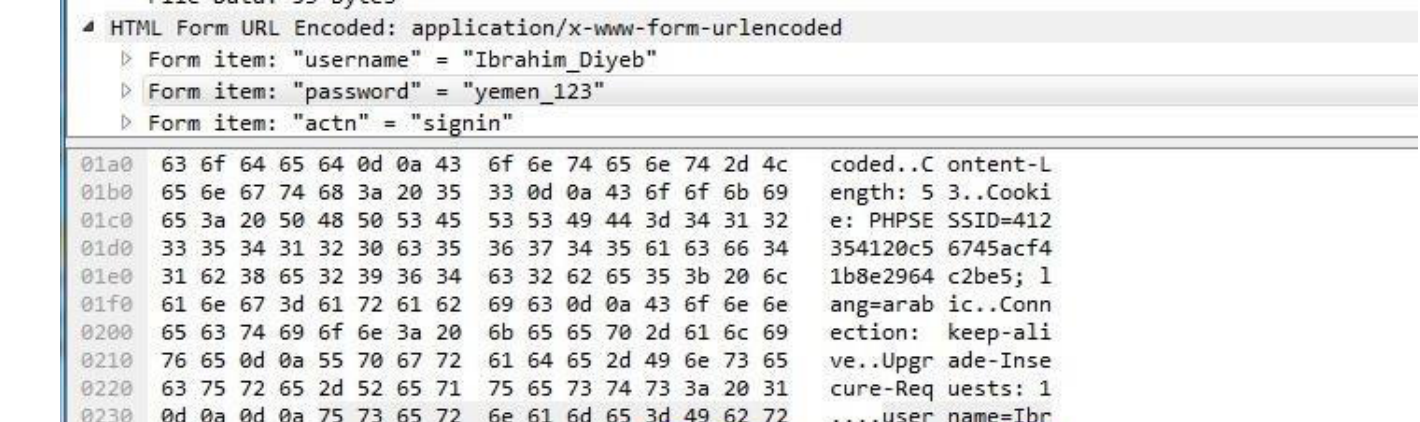
\includegraphics[width=0.9\linewidth, height=0.45\textheight, keepaspectratio]{figures/wireshark-plaintext.png}
    \caption{Tangkapan Wireshark pada lalu lintas HTTP yang tidak terenkripsi: nama pengguna dan kata sandi terbaca langsung tanpa perlu dipecahkan}
    \label{fig:wireshark-plaintext}
    \sumber{Munir, \textit{IF4020 Kriptografi}, ITB.}
\end{figure}

Selain penyadapan perangkat lunak di atas, terdapat tiga metode penyadapan yang
bekerja pada tingkat fisik.
\begin{enumerate}
    \item \textbf{Penyadapan kabel} (\textit{wiretapping}), yaitu menempelkan alat
          pada saluran komunikasi. Sistem telepon kabel sangat rentan terhadap cara
          ini karena rancangannya sederhana: di dalam kabel telepon standar hanya
          terdapat sepasang kawat yang membentuk rangkaian tertutup, sehingga
          menyisipkan penyadap hampir tidak mengubah perilaku rangkaian itu.
    \item \textbf{Penyadapan elektromagnetik} (\textit{electromagnetic
          eavesdropping}), yaitu menangkap radiasi elektromagnetik yang dipancarkan
          perangkat elektronik ketika bekerja. Dengan antena penerima sederhana,
          sinyal dari perangkat di ruangan sebelah dapat ditangkap dari jarak yang
          relatif dekat ($r < 2$ m), sebagaimana digambarkan pada
          Gambar~\ref{fig:penyadapan-elektromagnetik}. Perkakas radio berbasis
          perangkat lunak (\textit{software defined radio}) membuat cara ini makin
          mudah diakses.
    \item \textbf{Penyadapan akustik} (\textit{acoustic eavesdropping}), yaitu
          memanfaatkan getaran atau suara. Selain penyadapan langsung, terdapat
          teknik \textit{vibrometry} nirkabel yang menangkap getaran halus pada
          permukaan benda di ruangan korban, termasuk getaran yang ditimbulkan
          pengeras suara, sebagaimana ditunjukkan Gambar~\ref{fig:penyadapan-akustik}.
\end{enumerate}

\begin{figure}[htbp]
    \centering
    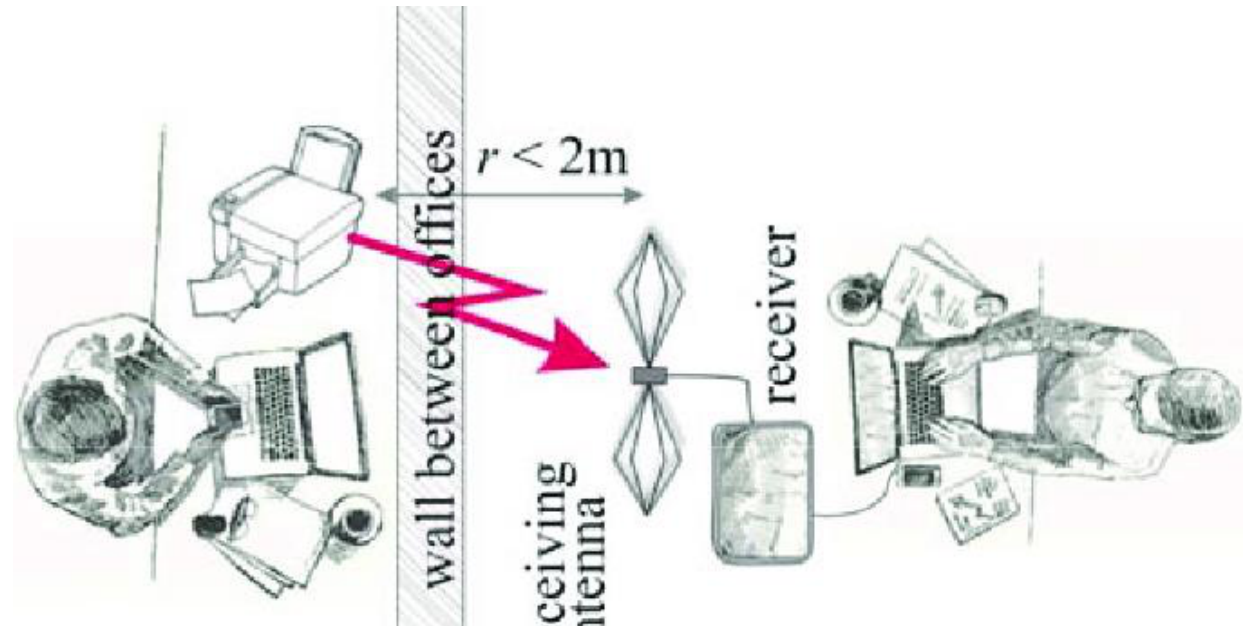
\includegraphics[width=0.78\linewidth, height=0.55\textheight, keepaspectratio]{figures/penyadapan-elektromagnetik.png}
    \caption{Penyadapan elektromagnetik: radiasi dari perangkat elektronik di ruangan sebelah ditangkap antena penerima dari jarak kurang dari dua meter}
    \label{fig:penyadapan-elektromagnetik}
    \sumber{Munir, \textit{IF4020 Kriptografi}, ITB.}
\end{figure}

\begin{figure}[htbp]
    \centering
    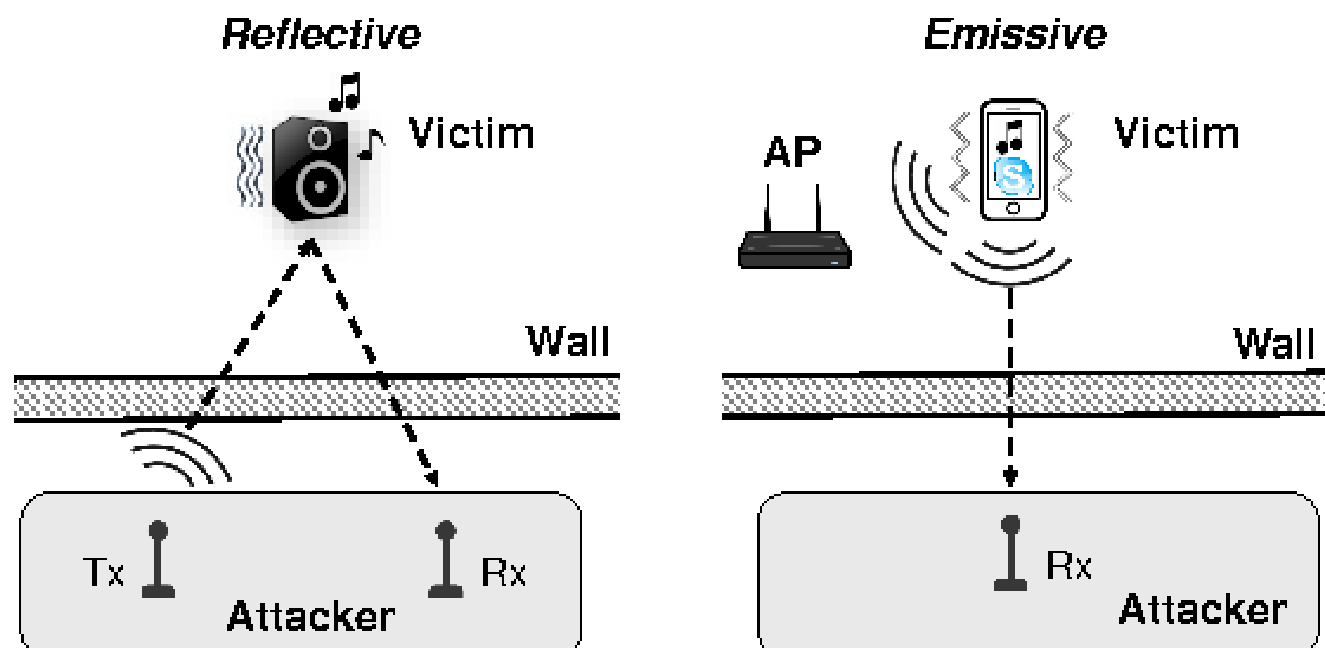
\includegraphics[width=0.85\linewidth, height=0.5\textheight, keepaspectratio]{figures/penyadapan-akustik.png}
    \caption{Penyadapan akustik melalui \textit{vibrometry} nirkabel: metode \textit{reflective} (kiri) dan \textit{emissive} (kanan) memanfaatkan getaran dari pengeras suara atau ponsel korban}
    \label{fig:penyadapan-akustik}
    \sumber{Munir, \textit{IF4020 Kriptografi}, ITB.}
\end{figure}

\subsection{Serangan Aktif (\textit{Active Attack})}

Penyerang mengintervensi komunikasi dan ikut memengaruhi sistem untuk keuntungan
dirinya. Ia dapat mengubah aliran pesan dengan menghapus sebagian cipherteks,
mengubah cipherteks, menyisipkan potongan cipherteks palsu, memutar ulang pesan
lama, atau mengubah informasi yang tersimpan. Contohnya adalah serangan
\textit{man-in-the-middle}.

Gambar~\ref{fig:serangan-mitm} menampilkan skema serangan MITM: koneksi asli antara
pengguna dan situs web diputus, lalu dialihkan melalui penyerang. Yang membuat
serangan ini berbahaya adalah bahwa kedua pihak sama-sama merasa berkomunikasi
langsung dengan pihak yang benar. Pada Bab~\ref{chap:diffie-hellman} akan
ditunjukkan bahwa protokol pertukaran kunci yang paling dasar pun rentan terhadap
serangan ini bila tidak dilengkapi mekanisme otentikasi.

\begin{figure}[htbp]
    \centering
    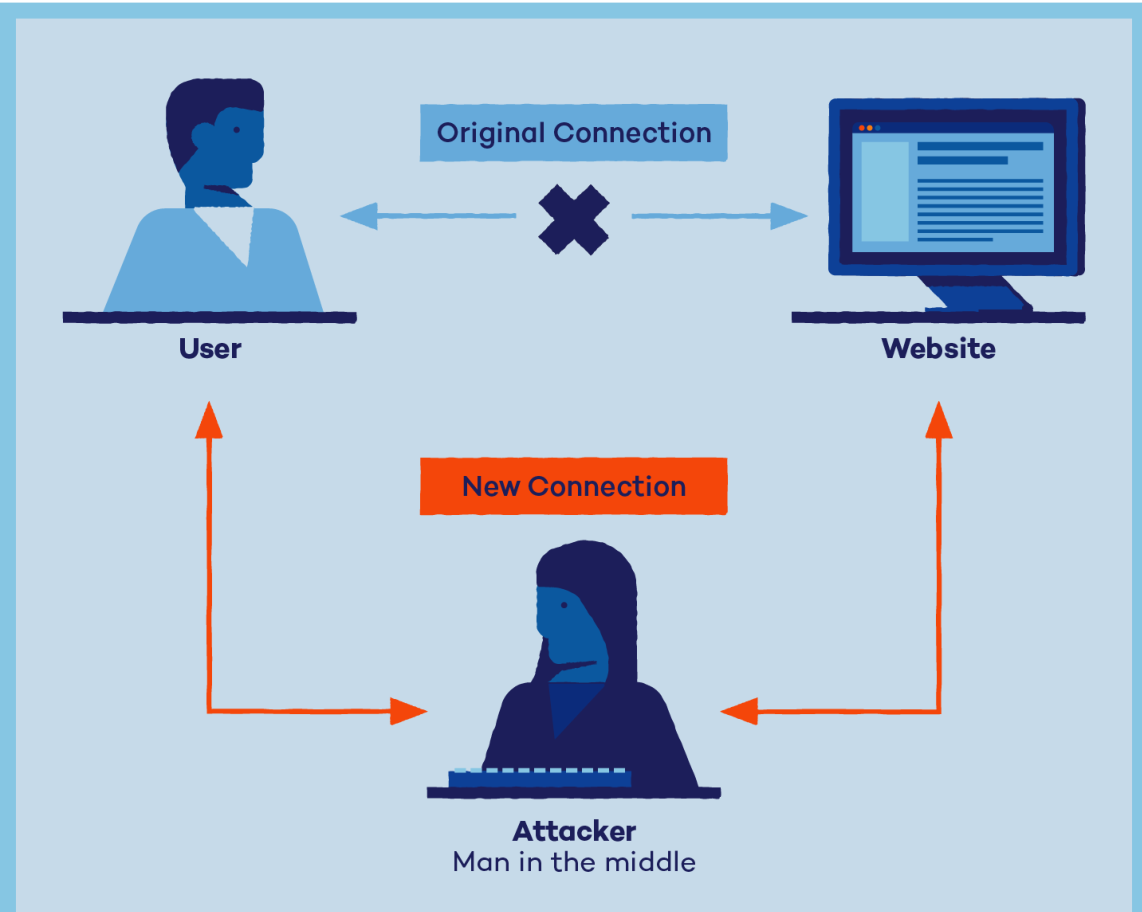
\includegraphics[width=0.7\linewidth, height=0.7\textheight, keepaspectratio]{figures/serangan-mitm.png}
    \caption{Serangan \textit{man-in-the-middle}: koneksi antara pengguna dan situs web diputus lalu dialihkan melalui penyerang}
    \label{fig:serangan-mitm}
    \sumber{Munir, \textit{IF4020 Kriptografi}, ITB.}
\end{figure}

Secara ringkas, ketujuh kategori serangan yang lazim dibicarakan dapat disusun
seperti pada Tabel~\ref{tab:kategori-serangan}. Pengelompokan pada tabel ini
mengikuti \citet{stallings2017}, dan pembedaan pasif--aktif di dalamnya sejalan
dengan pembahasan di atas.

\begin{table}[htbp]
    \centering
    \caption{Tujuh kategori serangan dan layanan keamanan yang terlanggar}
    \label{tab:kategori-serangan}
    \small
    \begin{tabularx}{\linewidth}{@{}l l >{\raggedright\arraybackslash}X >{\raggedright\arraybackslash}X@{}}
        \hline
        \textbf{Serangan} & \textbf{Kelas} & \textbf{Perbuatan penyerang} & \textbf{Contoh nyata} \\
        \hline
        Intersepsi & Pasif & Membaca isi pesan yang melintas &
        Menyadap kata sandi pada jaringan nirkabel terbuka \\
        \hline
        Analisis lalu lintas & Pasif & Mengamati pola dan volume komunikasi &
        Menyimpulkan aktivitas lembaga dari jadwal dan besar lalu lintas \\
        \hline
        Interupsi & Aktif & Memutus koneksi sehingga layanan tak tersedia &
        Serangan penolakan layanan terhadap peladen situs \\
        \hline
        Fabrikasi & Aktif & Mengirim pesan palsu yang tampak sah &
        Surel berisi instruksi transfer dengan pengirim palsu \\
        \hline
        Modifikasi & Aktif & Mengubah isi pesan di tengah jalan &
        Mengubah nomor rekening tujuan pada perintah pembayaran \\
        \hline
        Pemutaran ulang & Aktif & Mengirim ulang pesan sah yang pernah dicegat &
        Memutar ulang perintah transfer yang sama berkali-kali \\
        \hline
        \textit{Man-in-the-middle} & Aktif & Menyisipkan diri di antara kedua pihak &
        Memalsukan kunci publik pada pertukaran kunci Diffie--Hellman \\
        \hline
    \end{tabularx}
\end{table}
